\chapter{Applications of the Multi-flare Algorithm to Source Catalogs}\label{chapter:catalogsearches}
The multi-flare algorithm introduced in the previous section may be applied to an ensemble of sources that share common features. This is common practice in neutrino astronomy, as examining emission from a catalog allows us to explore the possibility of neutrino emission from a class of sources, rather than a specific individual source. 
Here, we explore two catalogs designed to explore source features related to those associated with the analysis of TXS 0506+056. Namely, the fact that the analysis was initially triggered by a high-energy neutrino event, and also the fact that TXS 0506+056 is a blazar. For the former, we assemble a catalog of high energy IceCube events to treat as "sources" (a "self-triggered" catalog analysis), while for the latter we use the pre-existing catalog of Fermi 3LAC blazars~\cite{fermi_3lac}.

In both cases, the multi-flare algorithm is applied at each source candidate location, resulting in a multi-flare test statistic (and corresponding pre-trial p-value) associated with each source candidate.
To test for potential sub-populations of strong emitters within the catalog, we additionally calculate a best-fit number of multi-flare sources via iteratively summing the sources with the largest test statistics (\ref{iterativesum}). For a given data set, the sources are ordered by their multiflare test statistic, $\widetilde{TS}$. A p-value for $k=1,2,3,...N_{srcs}$ is calculated, and subsequently the $k$ that produces the minimum p-value is selected ($k_{best}$).

\begin{equation}
    \widetilde{TS}_{all} = \sum_{m=0}^{k_{best}}\widetilde{TS}_m
\label{iterativesum}
\end{equation}

An additional trial factor is then calculated by applying this procedure to maps of data with randomized right ascension values to assemble a distribution of $\widetilde{TS}_{all}$ representative of the null hypothesis. A final p-value can then be obtained by comparing an observed $\widetilde{TS}_{all}$ with this null hypothesis distribution. 

For all the analyses detailed in this section, the NorthernTracksv002p05 sample was used. This sample is described earlier in this document (section 2.5). 

\section{Self-Triggered Catalog}
For this catalog, we select the locations of all the events in the NorthernTracks v002p05 data sample that have a reconstructed energy proxy greater than 200 TeV. This energy threshold is chosen as it is roughly the point where 50\% or more of neutrino events are expected to be astrophysical in origin. We can consequently expect that this catalog contains a non-negligible number of astrophysical neutrino sources, and can test the hypothesis of additional time dependent neutrino emission from these locations. Events that have been selected as source candidates for the catalog are subsequently removed from the sample, and do not otherwise contribute to the calculation of a multi-flare test statistic. 

This catalog contains 32 source candidates, all in the northern sky. Notably, this catalog does not include IC170922A (the alert event that triggered the followup analysis on TXS 0506+056), as the data sample does not extend past the 2015 season, and IC170922A occurred in the 2017 season. 

\begin{figure}[h]
\centering
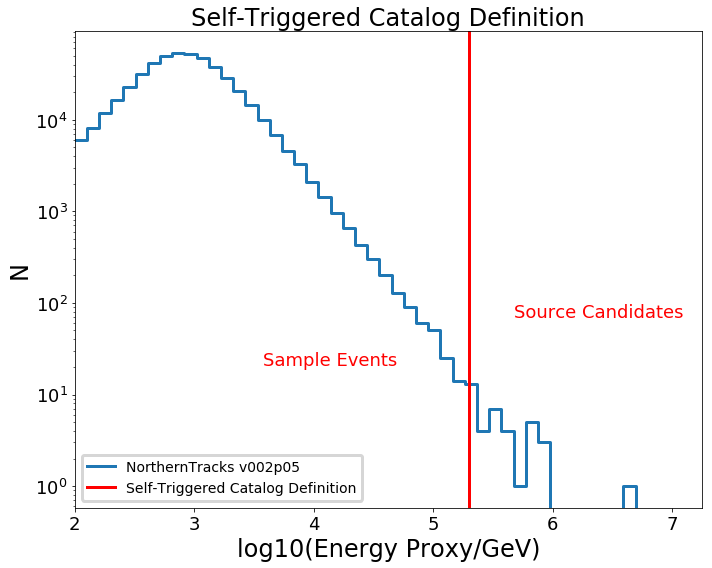
\includegraphics[width=0.4\textwidth]{figs/stcat_def.png}
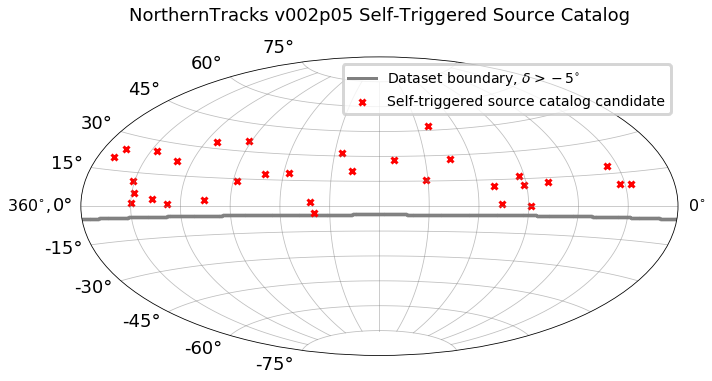
\includegraphics[width=0.4\textwidth]{figs/Selftriggeredcat.png}
\caption{Left: The self-triggered catalog definition: Events with energy proxies to the right of the vertical red line (200 TeV) are treated as source candidates. Events to the left of the red line are then investigated for clustering around the locations of the source candidate events. Right: The self-triggered catalog assembled from the NorthernTracks v002p05 data sample, consisting of all events in the sample with reconstructed energy proxy greater than 200 TeV. The locations of these events are treated as source candidates for the purposes of applying the multi-flare algorithm, however the events themselves are removed from the sample prior to calculating a test statistic.}
\label{fig:stcat}
\end{figure}

Applying the multi-flare algorithm described above to this catalog of the locations of 32 high energy neutrino events results in a best-fit number of sources of $k_{best}=4$, with an associated p-value of $p=0.017$ ($2.13\sigma)$, shown in figure~\ref{fig:stresults}. Detailed results for all 32 source candidates, including fitted number of events and pre-trial p-values, can be viewed in table~\ref{tab:stresults}. 

As mentioned in previous sections, a significant advantage of the multi-flare algorithm is the generation of neutrino "light curves" (or "flare curves") that show the historical activity of a source candidate. The flare curves associated with the 4 most significant sources in the self-triggered catalog can be seen in figure~\ref{fig:stcurves}.

\begin{figure}[h]
\centering
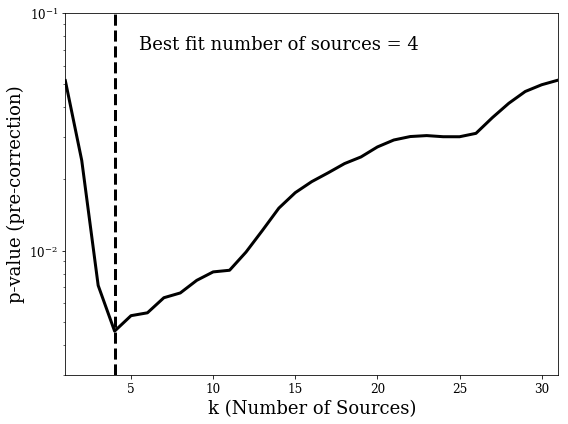
\includegraphics[width=0.4\textwidth]{figs/st_pcurve.png}
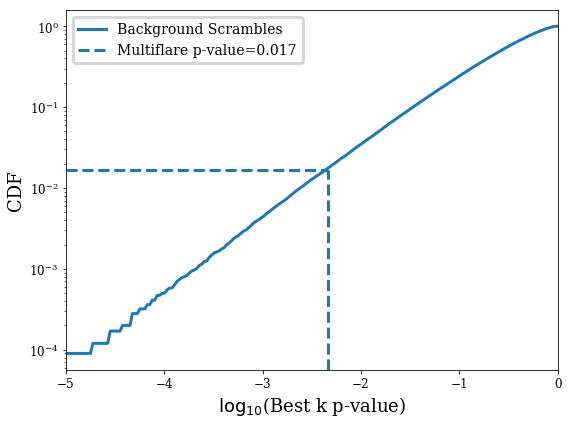
\includegraphics[width=0.4\textwidth]{figs/st_obsresult.png}
\caption{Left: The local significance of stacking the $k$ highest test statistic sources, as a function of $k$. The best fit value of $k=4$ can be seen as the minimum of this curve. Right: The trial corrected result for stacking the top 4 sources together, shown as a vertical line superimposed on the background distribution obtained by applying the algorithm to right-ascension scrambled data.}
\label{fig:stresults}
\end{figure}

\begin{table}[h!]
\centering
 \begin{tabular}{||c c c c||} 
 \hline
 RA & Dec & $\hat{n}_s$ & $p$ (pre-trial) \\ [0.5ex] 
 \hline\hline
 36.69 & 18.32 & 47.21 & 0.00197 \\ 
 \hline
 272.14 & 35.66 & 30.71 & 0.00729 \\
 \hline
 170.19 & 27.85 & 45.75 & 0.00834 \\
 \hline
 93.26 & 16.33 & 30.02 & 0.02667 \\
 \hline
\end{tabular}
\caption{The top 4 most significant multi-flare source candidates in the self-triggered catalog composed of high energy IceCube neutrino events. Collectively, these sources form an excess with a significance of $p=0.017$.}
\label{tab:stresults}
\end{table}


\begin{figure}[h]
\centering
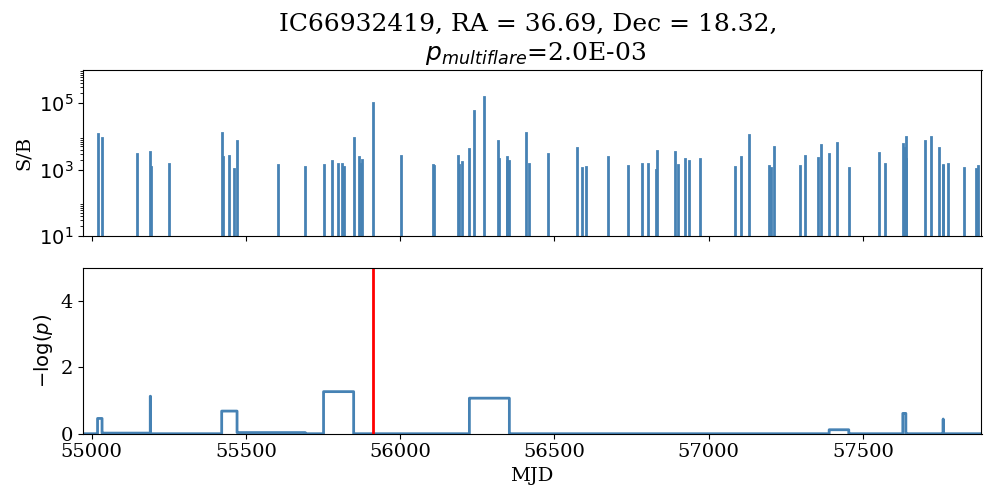
\includegraphics[width=0.4\textwidth]{figs/66932419.png}
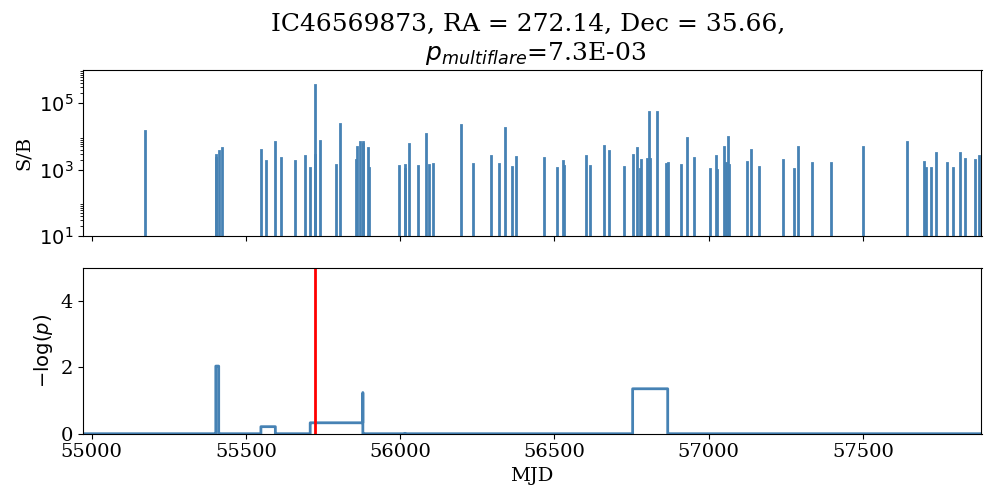
\includegraphics[width=0.4\textwidth]{figs/46569873.png}
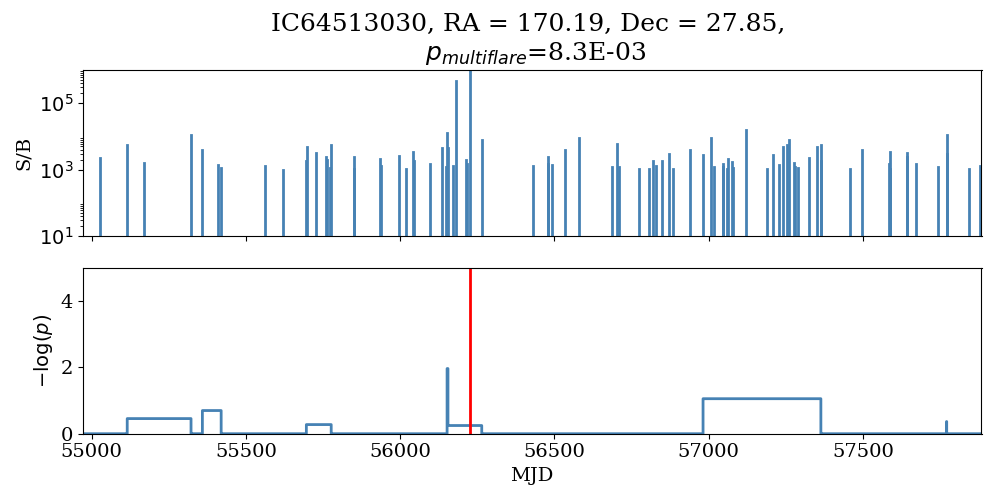
\includegraphics[width=0.4\textwidth]{figs/64513030.png}
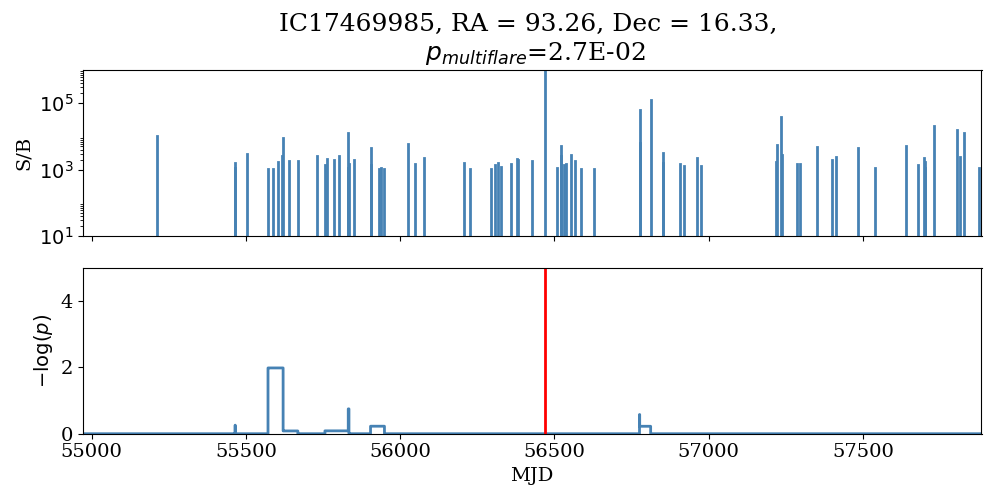
\includegraphics[width=0.4\textwidth]{figs/17469985.png}
\caption{The neutrino "flare curves" associated with the 4 most significant multiflare source candidates in the self-triggered catalog. The top panel of each subplot shows the event weights, calculated by taking the ratio of the spatial and energy components of the signal and background PDFs described in equation~\ref{spaceEcomponents_sig} and \ref{spaceEcomponents_bg}, while the bottom panels show the fitted ensemble of decorrelated flares, with the local per-flare p-value plotted on the y-axis. The vertical red line denotes the arrival time of the high energy event used to define the source candidate location. This event is removed from the sample prior to applying the multiflare-algorithm, and consequently these events do not contribute to the flare curves shown in this figure.}
\label{fig:stcurves}
\end{figure}


Though not statistically significant, these results have several interesting features. Though the high-energy "seed" events are removed prior to the calculation of a flare curve, 7 of the flare curves generated include flares that would have included a high energy seed event. Though not statistically significant, this is certainly above average, as only 11\% of background trials have 7 or more flare curves with seed event/flare correlations. 


\begin{figure}[h]
\centering
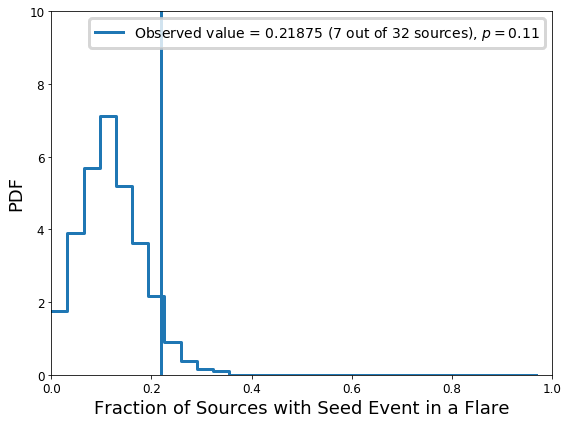
\includegraphics[width=0.8\textwidth]{figs/evtflarecorr.png}
\caption{The distribution of number of flare curves that have a temporal correlation between the high energy seed event, and a fitted flare, obtained from sets of data where the right ascension of events has been randomized. The observed value (7 out of 32 sources, or 21.9\%) is shown as a blue vertical line. 11\% of trials have more than 7 correlations between seed events and fitted flares.}
\label{fig:stresults}
\end{figure}

It is also potentially interesting to investigate the distributions of the parameters fit by the multi-flare likelihood. By comparing the observed distributions with those expected from background scrambles, we can check for inconsistencies of our data with the null hypothesis. 

\begin{figure}[h]
\centering
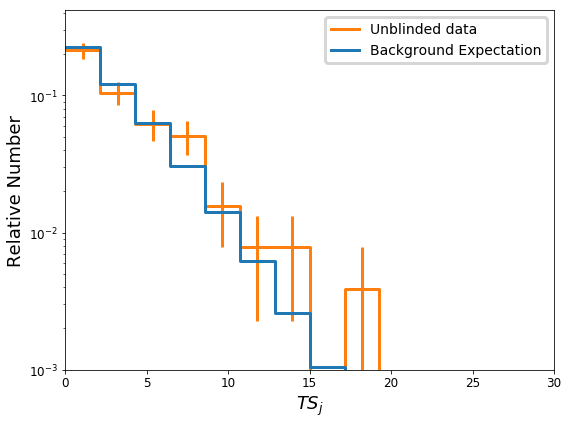
\includegraphics[width=0.4\textwidth]{figs/st_tsjdist.png}
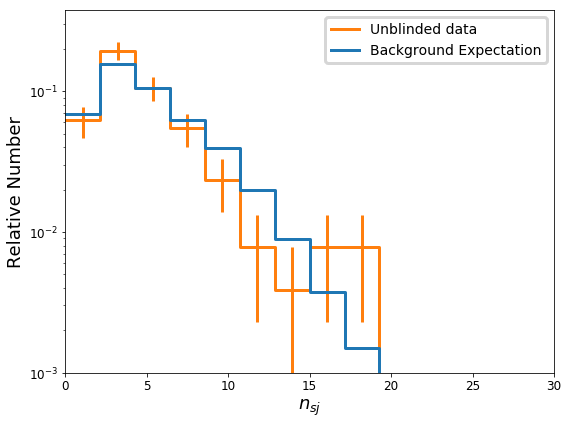
\includegraphics[width=0.4\textwidth]{figs/st_nsdist.png}
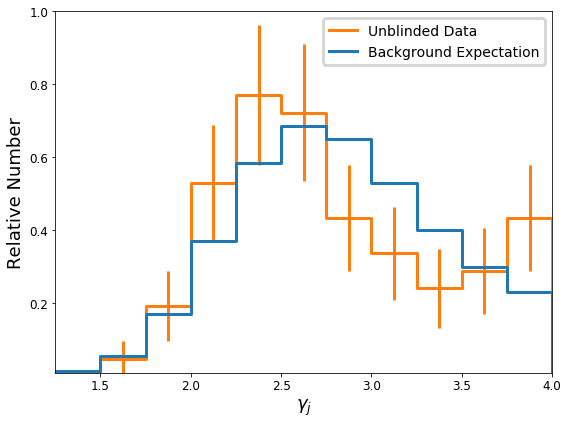
\includegraphics[width=0.4\textwidth]{figs/st_gammadist.png}
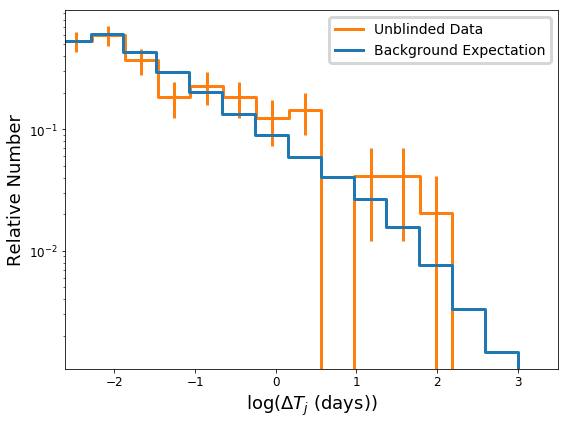
\includegraphics[width=0.4\textwidth]{figs/st_dtdist.png}
\caption{Distributions of fitted flare parameters for flares associated with the self-triggered catalog in both background scrambles (blue) and unblinded data (orange). While there is potentially some deformation in the distribution of fitted spectral indices (bottom left), a 2-sample K-S test comparing the observed and background distributions only returns a p-value of $p=0.26$, indicating that the blue and the orange distributions are not significantly inconsistent with one another. }
\label{fig:stresults}
\end{figure}

\section{Fermi 3LAC Blazars}
The 2014 TXS 0506+056 neutrino flare was notable not only for its association with a high energy IceCube alert, but also for its spatial coincidence with the blazar TXs 0506+056. In searching for additional neutrino sources, it is then not unreasonable to assemble a search for neutrino flares associated with a large catalog of blazars. For this purpose, we use the Fermi 3LAC catalog~\cite{fermi_3lac} to define a set of source candidates. Previous analyses searching for spatial coincidence with earlier iterations of this catalog have been performed, but were unable to identify any statistically significant excess~\cite{2lac_ic}. Here, we instead specifically search for transient emission using multi-flare algorithm described above. 

The Fermi 3LAC catalog is a catalog of AGNs detected by Fermi-LAT, consisting of gamma ray sources in the third Fermi-LAT catalog (3FGL)~\cite{fermi3fgl} between 100 MeV and 300 GeV with a Fermi test statistic greater than 25 between August 4, 2008, and July 31, 2012~\cite{fermi_3lac}. The catalog contains 1591 objects, the majority (98\%) of which are blazars, roughly evenly split between FSRQs and BL Lacs. Notably, TXS 0506+056 is a member of this catalog. 

In constructing this analysis, we select for blazars at declinations greater than $-5^{\circ}$, as the IceCube data sample (NorthernTracks v002p05) does not extend below this point. We impose no further cuts, and all sources are weighted equally when calculating a multi-flare test statistic. The final catalog to be used for the multi-flare analysis consists of 1023 blazars, the locations of which are shown in figure~\ref{fig:3laccat}.

\begin{figure}[h]
\centering
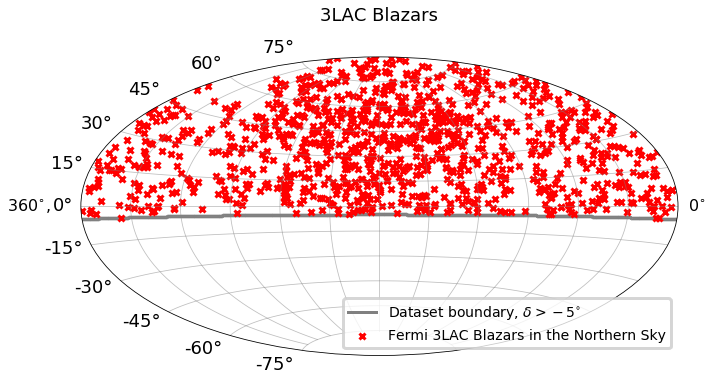
\includegraphics[width=0.8\textwidth]{figs/3lac_skymap.png}
\caption{The locations of the 3LAC blazars that compose the catalog used for a multi-flare analysis. Blazars with $\delta<5^{\circ}$ are not considered, as the IceCube NorthernTracks v002p05 data sample does not extend into this region. There are 1023 blazars that are considered as source candidates for the multi-flare analysis.}
\label{fig:3laccat}
\end{figure}

The results of applying the multi-flare algorithm to this catalog of 3LAC blazars can be summarized in figure~\ref{fig:3lacresults}. The optimization procedure for the most significant combination of sources returned a best fit number of sources of $k=125$, with an associated post-trial p-value of $p=0.06$. A list of these source candidates can be seen in table~\ref{tab:3lacresults}. As the significance of this excess is consistent with the null hypothesis, we do not claim discovery of neutrino flares associated with 3LAC blazars. 

Interestingly, despite the presence of the 2014 neutrino flare identified in~\cite{TXS_Archival}, TXS 0506+056 is not the most significant source candidate, having a pre-trial p-value of only $p=9.24 \times 10^{-3}$. This is not unexpected, considering that there does not appear to much activity (in terms of neutrino flares) at this location beyond the 2014 flare itself. As the multi-flare algorithm performs will return a high significance when there are multiple, moderately significant flares to stack together, it is unsurprising that there are other sources that have a higher multi-flare significance. As an example, the source candidate with the highest multi-flare significance is 1RXS J154604.6+081912. Rather than having a single large flare, the multi-flare algorithm fits multiple flares at this source candidate location, which combined have a significance of $p=8.1 \times 10^{-5}$, despite none of the individual flares having a local significance much greater than $p=0.01$.

\begin{figure}[h]
\centering
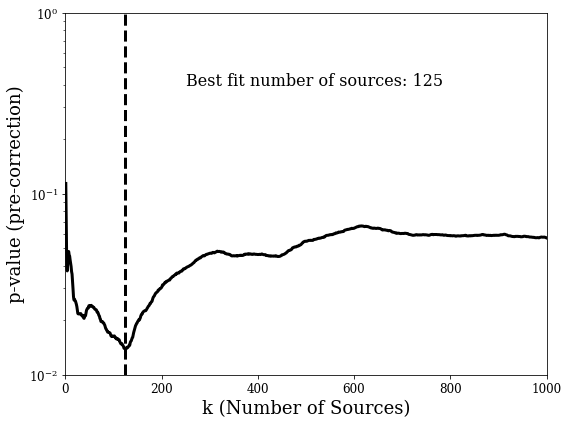
\includegraphics[width=0.4\textwidth]{figs/3lac_pcurve.png}
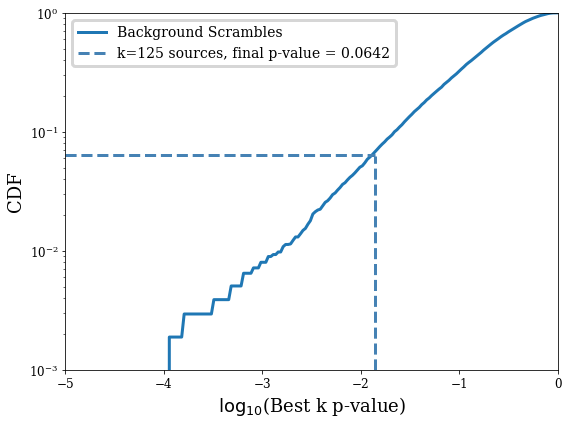
\includegraphics[width=0.4\textwidth]{figs/3lacresult.png}
\caption{Left: The local significance of stacking the $k$ highest test statistic sources in the 3LAC blazar catalog, as a function of $k$. The best fit value of $k=125$ can be seen as the minimum of this curve. Right: The trial corrected result for stacking the top 125 sources together, shown compared the background distribution obtained by applying the algorithm to right-ascension scrambled data. As the final p-value associated with the top 125 blazar sources is only $p=0.06$, there was no significant excess of neutrino flares observed to be associated with 3LAC blazars.}
\label{fig:3lacresults}
\end{figure}

Similar to the self-triggered catalog, we can additionally examine the distributions of the flare parameters that were fit for all the sources in the 3LAC catalog. No significant deviations from the background expectation are observed in any of the flare parameter distributions, as seen in figure~\ref{fig:3lacresults}.

As with the self-triggered catalog, we also obtain neutrino flare curves describing the historical variability of each source candidate. Figure~\ref{fig:3lacflarecurves} shows the flare curves of several 3LAC source candidates of note, including TXS 0506+056. While none of these sources are significant enough to claim discovery, flare curves like the ones shown here are a potentially valuable tool for multi-messenger analyses in the future that may seek to correlate neutrino emission with other astrophysical messengers. 

Though the application of the multi-flare algorithm to this catalog of 3LAC blazars did not result in a significant detection, it does allow us to constrain the behavior of neutrino flares associated with 3LAC blazars. Given that this method stacks flares together, the lack of a significant results suggest that there is an upper limit to how bright and numerous blazar neutrino flares may be. We express these limits in terms of the flare rate (how many flares occurred over the livetime of the data sample), and the per-flare $E^2$ flux. This allows us to compare to previously calculated limits obtained from a time-integrated analysis~\cite{2lac_ic}. These upper limits can be seen in figure~\ref{fig:3laclims}

\begin{figure}[h]
\centering
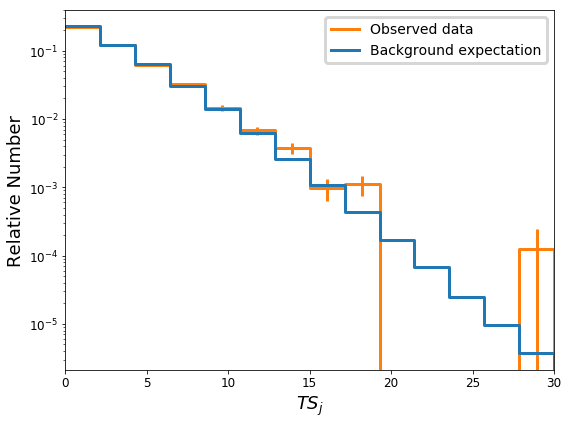
\includegraphics[width=0.4\textwidth]{figs/3lac_tsjs.png}
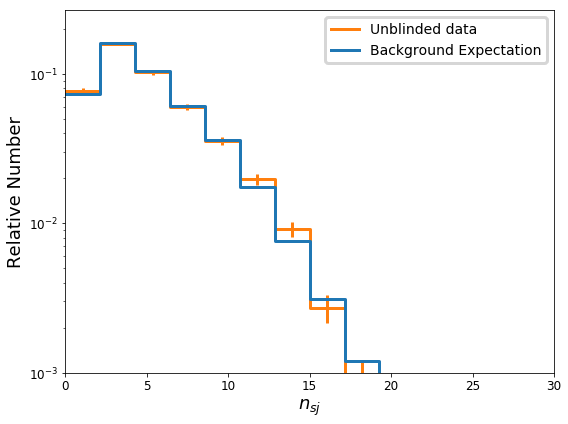
\includegraphics[width=0.4\textwidth]{figs/3lac_nss.png}
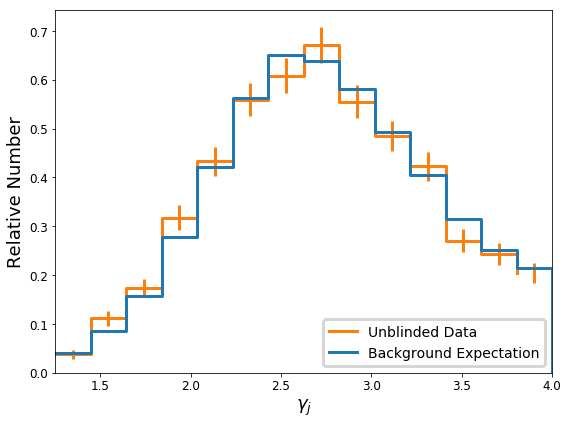
\includegraphics[width=0.4\textwidth]{figs/3lac_gammas.png}
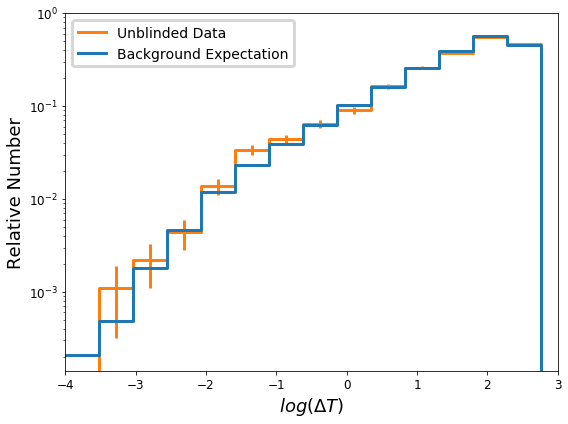
\includegraphics[width=0.4\textwidth]{figs/3lac_dts.png}
\caption{Distributions of fitted flare parameters for flares associated with the 3LAC blazar catalog in both background scrambles (blue) and unblinded data (orange). All distributions of fit parameters from observed data appear to be consistent with the background expectation. As this catalog includes TXS 0506+056, the 2014 neutrino flare originally discovered in the IC170922A follow-up analysis~\cite{TXS_Archival} is visible as the rightmost entry in the histogram of flare $TS_j$ values in the plot in the upper left, having a value of $TS_j=27.9$. There are no other flares that were fit in this catalog with $TS_j>20$. }
\label{fig:3lacresults}
\end{figure}

\begin{figure}[h]
\centering
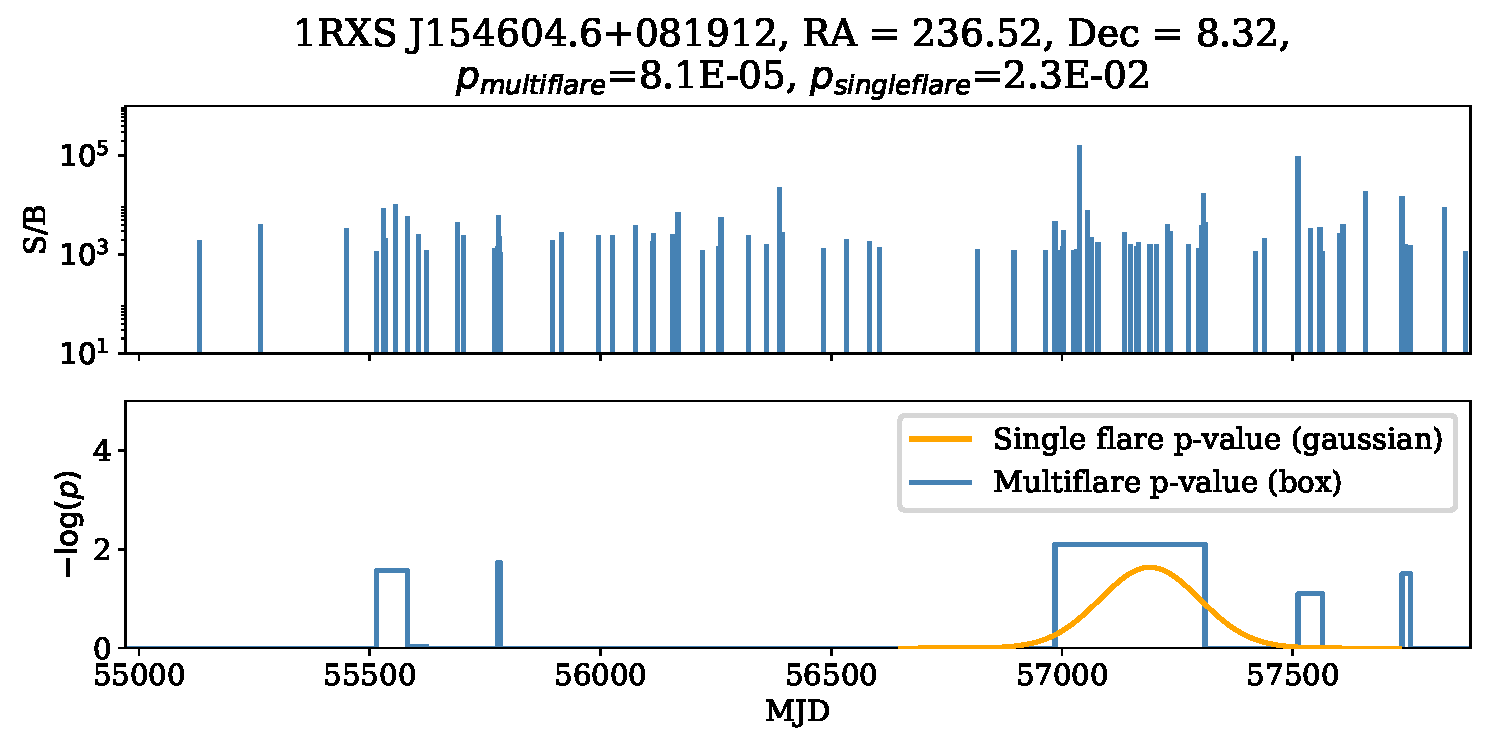
\includegraphics[width=0.44\textwidth]{figs/1RXS J154604.6+081912.pdf}
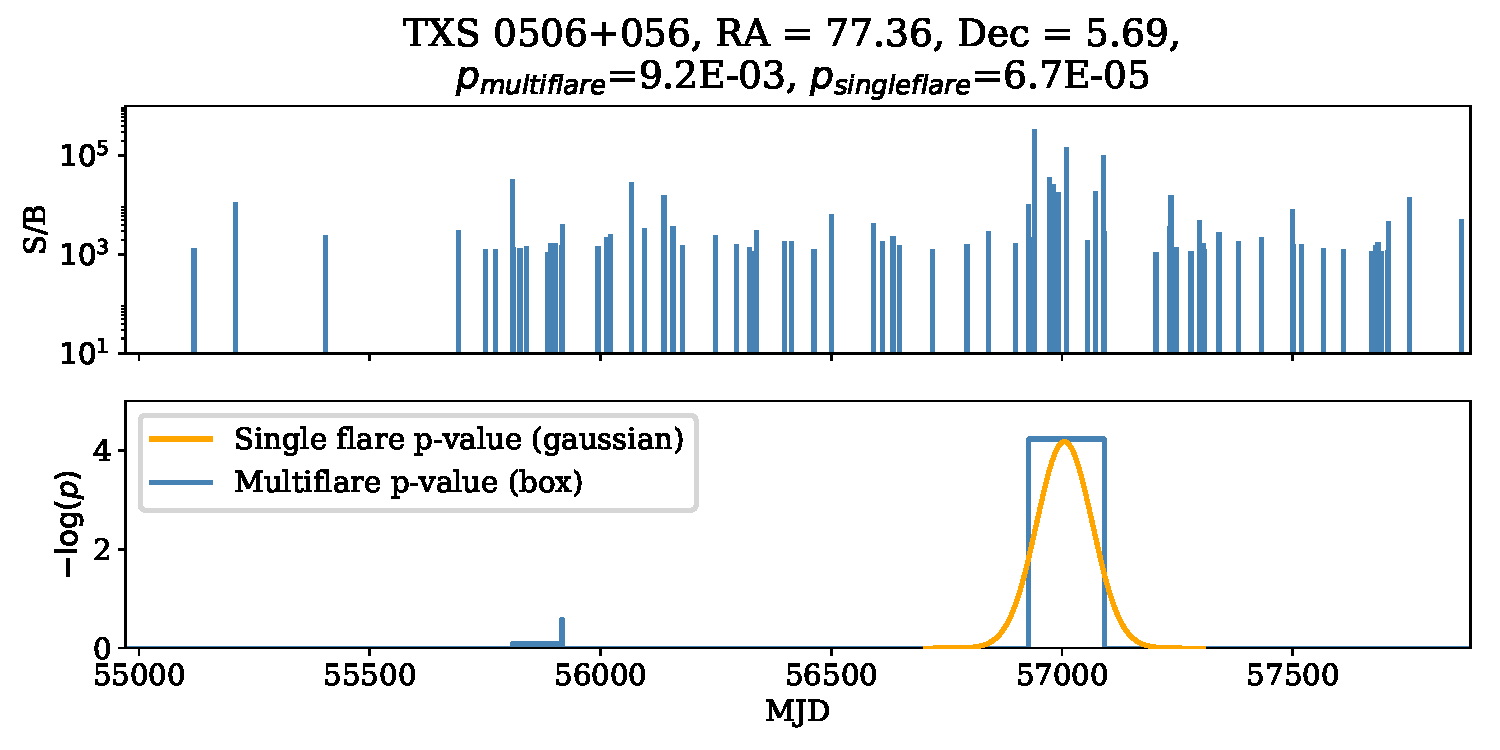
\includegraphics[width=0.44\textwidth]{figs/TXS 0506+056.pdf}
\caption{Neutrino flare curves for several sources of note in the multi-flare 3LAC blazar catalog analysis. The flare curves generated by the multi-flare algorithm are shown in blue, while the results of a corresponding single-flare analysis (that only fits the largest flare on each source) are shown in orange. Left: 1RXS J154604.6+081912, the most significant 3LAC blazar in the multi-flare analysis, having a pre-trial multi-flare p-value of $p=8.11 \times 10^{-5}$. Note that for this particular source, the multi-flare significance driven by a set of five moderately significant flares, none of which are particularly significant on their own. The significance of this source in the single-flare analysis was only $p=0.02$. Right: The flare curve for TXS 0506+056, showing the sizeable 2014 neutrino flare originally observed in~\cite{TXS_Archival}. The multi-flare p-value for TXS 0506+056 is only $p=9.24 \times 10^{-3}$, as other than the 2014 neutrino flare, there are no other particularly significant neutrino flare candidates at this location. }
\label{fig:3lacflarecurves}
\end{figure}

\begin{figure}[h]
\centering
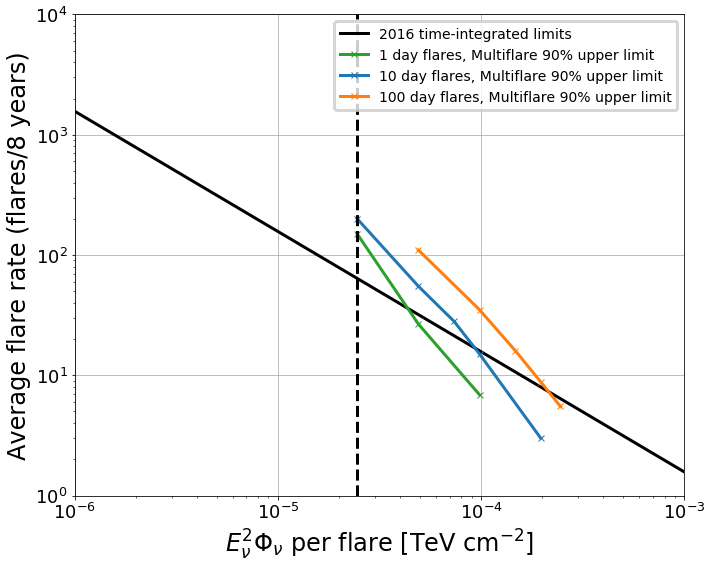
\includegraphics[width=0.8\textwidth]{figs/3lac_lims.png}
\caption{The 90\% upper limits associated with the non-detection of a multi-flare signal using the 3LAC blazar catalog. The solid black line represents the time integrated limits obtained from ~\cite{2lac_ic}. Colored curves represent limits associated with various flare durations, as the multi-flare method imposes more stringent limits in the case that flares are shorter (for a fixed $E^2$ flux per flare). Note that the parameter space that is realistically accessible to a time-dependent analysis is somewhat compressed: points below the x-axis do not produce more than 1 flare in the data sample, on average, and points to the left of the vertical dashed line have an average flare size of $< 1$ event.}
\label{fig:3laclimits}
\end{figure}


%\captionsetup{width=20cm}
\begin{center}
\label{tab:3lacresults}
\begin{longtable}{||cccccc||}
\caption{The top 125 multiflare source candidates in the 3LAC blazar catalog.}\\
\hline
Source Candidate Name & Source Class & RA (deg) & Dec (deg) & $\hat{n}_s$ & $p$ (pre-trial)\\
\hline
\endfirsthead
\multicolumn{6}{c}%
{\tablename\ \thetable\ -- \textit{Continued from previous page}} \\
\hline
Source Candidate & Source Class & RA (deg) & Dec (deg) & $\hat{n}_s$ & $p$ (pre-trial) \\
\hline
\endhead
\hline \multicolumn{4}{r}{\textit{Continued on next page}} \\
\endfoot
\hline
\endlastfoot
1RXS J154604.6+081912 &  bll  & 236.52 & 8.32 & 53.49 & 8.11e-5  \\
RBS 1467 &  bll  & 227.18 & 27.15 & 55.11 & 3.05e-4  \\
GB6 J0723+2859 &  fsrq  & 110.98 & 28.99 & 40.48 & 4.58e-4  \\
RBS 1558 &  bll  & 241.59 & 56.51 & 28.88 & 1.92e-3  \\
PMN J2324+0801 &  bll  & 351.19 & 8.04 & 28.15 & 3.11e-3  \\
B2 2214+24B &  bll  & 334.25 & 24.36 & 36.90 & 3.79e-3  \\
GB6 J0850+4855 &  bll  & 132.50 & 48.92 & 38.18 & 4.75e-3  \\
4C +20.25 &  fsrq  & 171.49 & 20.10 & 27.83 & 5.02e-3  \\
MG2 J094148+2728 &  fsrq  & 145.45 & 27.48 & 60.58 & 5.12e-3  \\
TXS 2241+406 &  bll  & 341.05 & 40.95 & 22.61 & 5.23e-3  \\
TXS 0213+619 &  bcu III  & 34.26 & 62.19 & 30.15 & 5.32e-3  \\
GB6 J0100+0745 &  bll  & 15.09 & 7.76 & 37.33 & 6.45e-3  \\
RX J0850.5+3455 &  bll  & 132.65 & 34.92 & 20.42 & 7.16e-3  \\
B2 1436+37B &  fsrq  & 219.72 & 37.18 & 49.47 & 7.83e-3  \\
MG1 J165034+0824 &  fsrq  & 252.66 & 8.41 & 39.19 & 7.83e-3  \\
PKS 0256+075 &  fsrq  & 44.86 & 7.79 & 42.53 & 9.04e-3  \\
TXS 0506+056 &  bll  & 77.36 & 5.69 & 20.71 & 9.24e-3  \\
1ES 1421+582 &  bll  & 215.66 & 58.03 & 28.49 & 0.0100  \\
TXS 0518+211 &  bll  & 80.44 & 21.21 & 48.49 & 0.0118  \\
W Comae &  bll  & 185.38 & 28.23 & 30.32 & 0.0123  \\
NVSS J141828+354250 &  bcu II  & 214.62 & 35.71 & 40.74 & 0.0128  \\
PKS 1532+01 &  fsrq  & 233.72 & 1.52 & 30.78 & 0.0131  \\
PKS 1424+240 &  bll  & 216.75 & 23.80 & 52.78 & 0.0148  \\
B3 2319+444 &  fsrq  & 350.58 & 44.76 & 41.93 & 0.0160  \\
PKS 0039+230 &  fsrq  & 10.52 & 23.33 & 48.89 & 0.0168  \\
B3 2238+410 &  bll  & 340.28 & 41.34 & 21.24 & 0.0175  \\
TXS 2315+189 &  bcu II  & 349.60 & 19.25 & 31.98 & 0.0197  \\
B3 2322+396 &  bll  & 351.32 & 39.96 & 30.07 & 0.0199  \\
NVSS J080637+774607 &  bcu II  & 121.66 & 77.77 & 52.32 & 0.0215  \\
MG1 J010908+1816 &  bll  & 17.28 & 18.27 & 26.59 & 0.0220  \\
1H 0323+342 &  nlsy1  & 51.17 & 34.18 & 10.09 & 0.0221  \\
NVSS J131921+775823 &  bcu II  & 199.84 & 77.97 & 16.99 & 0.0224  \\
RX J1351.3+1115 &  bll  & 207.84 & 11.25 & 27.93 & 0.0228  \\
RGB J1808+468 &  bll  & 272.00 & 46.83 & 29.19 & 0.0252  \\
RX J1149.5+2439 &  bll  & 177.38 & 24.66 & 33.52 & 0.0266  \\
TXS 2157+102 &  bll  & 330.03 & 10.50 & 47.04 & 0.0271  \\
S5 1357+76 &  fsrq  & 209.48 & 76.72 & 35.44 & 0.0274  \\
S5 1803+784 &  bll  & 270.19 & 78.47 & 27.73 & 0.0287  \\
GB6 J1439+4958 &  bll  & 219.95 & 49.97 & 32.32 & 0.0291  \\
B2 2234+28A &  bll  & 339.09 & 28.48 & 25.36 & 0.0298  \\
GB6 J0929+5013 &  bll  & 142.31 & 50.23 & 20.09 & 0.0306  \\
RGB J2054+002 &  bll  & 313.74 & 0.26 & 26.79 & 0.0315  \\
1ES 1028+511 &  bll  & 157.83 & 50.89 & 35.27 & 0.0333  \\
GB6 J0331+6307 &  bcu II  & 52.97 & 63.14 & 26.86 & 0.0335  \\
PKS 2320-035 &  fsrq  & 350.88 & -3.28 & 15.57 & 0.0350  \\
GB6 J0934+3926 &  bll  & 143.53 & 39.44 & 32.46 & 0.0352  \\
B2 1811+31 &  bll  & 273.40 & 31.74 & 35.37 & 0.0356  \\
GB6 J0937+5008 &  fsrq  & 144.30 & 50.15 & 27.81 & 0.0357  \\
TXS 1015+057 &  fsrq  & 154.62 & 5.51 & 19.30 & 0.0361  \\
TXS 1614+473 &  fsrq  & 243.92 & 47.19 & 16.66 & 0.0374  \\
4C +04.42 &  fsrq  & 185.59 & 4.22 & 19.22 & 0.0376  \\
MG2 J110606+2812 &  fsrq  & 166.53 & 28.21 & 41.99 & 0.0396  \\
RX J1246.9+4423 &  bll  & 191.75 & 44.39 & 22.30 & 0.0396  \\
B2 2308+34 &  fsrq  & 347.77 & 34.42 & 41.08 & 0.0408  \\
TXS 2106-030 &  bll  & 317.19 & -2.84 & 16.86 & 0.0410  \\
NVSS J125820+612049 &  bll  & 194.59 & 61.35 & 36.36 & 0.0425  \\
SBS 0812+578 &  bll  & 124.09 & 57.65 & 41.15 & 0.0426  \\
WN B1609.6+8517 &  bcu II  & 240.13 & 85.16 & 37.14 & 0.0434  \\
PMN J2227+0037 &  bll  & 336.99 & 0.62 & 28.56 & 0.0440  \\
1RXS J234332.5+343957 &  bll  & 355.89 & 34.66 & 25.27 & 0.0440  \\
GB6 J0529+0934 &  bcu II  & 82.26 & 9.58 & 32.69 & 0.0450  \\
MG2 J131037+2447 &  bcu III  & 197.66 & 24.81 & 27.71 & 0.0458  \\
3C 454.3 &  fsrq  & 343.49 & 16.15 & 37.56 & 0.0459  \\
GB6 J0929+7304 &  bcu II  & 142.43 & 73.07 & 25.62 & 0.0459  \\
ZS 0214+083 &  bll  & 34.32 & 8.62 & 36.08 & 0.0485  \\
3C 264 &  rdg  & 176.27 & 19.61 & 36.47 & 0.0485  \\
RXS J094620.5+010459 &  bll  & 146.58 & 1.08 & 19.50 & 0.0486  \\
NRAO 512 &  fsrq  & 250.12 & 39.78 & 21.52 & 0.0490  \\
1H 0323+022 &  bll  & 51.56 & 2.42 & 43.87 & 0.0494  \\
GB6 J1027+7428 &  bcu II  & 156.85 & 74.47 & 31.92 & 0.0495  \\
RX J0805.4+7534 &  bll  & 121.36 & 75.57 & 30.25 & 0.0505  \\
4C +73.07 &  bcu II  & 142.25 & 72.95 & 22.60 & 0.0514  \\
B3 1222+438 &  bll  & 186.21 & 43.59 & 28.13 & 0.0516  \\
MG1 J120448+0408 &  fsrq  & 181.22 & 4.14 & 33.72 & 0.0525  \\
GB6 J0148+5202 &  bcu III  & 27.08 & 52.03 & 19.63 & 0.0556  \\
7C 1823+6856 &  bll  & 275.89 & 68.96 & 21.57 & 0.0561  \\
MG2 J180948+2910 &  bll  & 272.44 & 29.17 & 34.89 & 0.0591  \\
NVSS J022304+682154 &  bcu II  & 35.77 & 68.37 & 31.49 & 0.0591  \\
OM 280 &  bll  & 177.58 & 24.30 & 42.49 & 0.0626  \\
PKS 1717+177 &  bll  & 259.80 & 17.75 & 24.64 & 0.0627  \\
1RXS J133021.4+444117 &  bll  & 202.59 & 44.69 & 22.24 & 0.0650  \\
S4 1726+45 &  fsrq  & 261.87 & 45.51 & 34.78 & 0.0664  \\
RX J1702.6+3115 &  bll  & 255.66 & 31.26 & 25.34 & 0.0664  \\
SBS 1410+530 &  bcu I  & 212.96 & 52.82 & 24.04 & 0.0666  \\
MG1 J154628+1817 &  bll  & 236.60 & 18.29 & 40.11 & 0.0668  \\
MG2 J190411+3627 &  bcu II  & 286.05 & 36.45 & 34.19 & 0.0713  \\
TXS 2331+073 &  fsrq  & 353.55 & 7.61 & 27.29 & 0.0731  \\
PKS 2047+098 &  bcu II  & 312.44 & 10.05 & 19.18 & 0.0734  \\
GB6 J1542+6129 &  bll  & 235.74 & 61.50 & 34.32 & 0.0736  \\
S5 0159+723 &  bll  & 30.89 & 72.55 & 30.54 & 0.0765  \\
TXS 2032+117 &  fsrq  & 308.65 & 11.91 & 21.51 & 0.0777  \\
S5 1027+74 &  bcu I  & 157.84 & 74.70 & 30.89 & 0.0777  \\
RGB J1426+340 &  bll  & 216.53 & 34.07 & 45.49 & 0.0778  \\
B3 0350+465 &  bcu III  & 58.63 & 46.72 & 22.88 & 0.0778  \\
RGB J1742+597 &  bll  & 265.63 & 59.75 & 37.12 & 0.0781  \\
1RXS J125117.4+103914 &  bll  & 192.82 & 10.65 & 18.18 & 0.0782  \\
MG3 J184126+2910 &  bcu II  & 280.34 & 29.16 & 37.55 & 0.0787  \\
TXS 1645+635 &  fsrq  & 251.49 & 63.50 & 36.91 & 0.0793  \\
B3 1058+413 &  bcu III  & 165.35 & 41.06 & 44.91 & 0.0799  \\
87GB 152947.5+574636 &  bll  & 232.74 & 57.61 & 21.01 & 0.0802  \\
GB6 J0229+6706 &  bcu III  & 37.34 & 67.11 & 11.03 & 0.0806  \\
MG1 J125348+0326 &  bll  & 193.45 & 3.44 & 27.69 & 0.0806  \\
GB6 J0342+3858 &  fsrq  & 55.57 & 38.99 & 33.59 & 0.0806  \\
PMN J0148+0129 &  bll  & 27.14 & 1.48 & 18.43 & 0.0818  \\
87GB 164812.2+524023 &  bll  & 252.35 & 52.59 & 33.97 & 0.0827  \\
GB6 J0024+0349 &  fsrq  & 6.19 & 3.82 & 31.06 & 0.0830  \\
B3 1307+433 &  bll  & 197.36 & 43.08 & 22.38 & 0.0839  \\
NVSS J092542+595812 &  bll  & 141.43 & 59.97 & 17.27 & 0.0913  \\
TXS 1549+089 &  bll  & 238.01 & 8.85 & 30.66 & 0.0915  \\
RX J0202.9-0223 &  bcu II  & 30.72 & -2.39 & 11.81 & 0.0922  \\
PKS 1203+04 &  ssrq  & 181.58 & 4.10 & 39.00 & 0.0926  \\
3C 221 &  rdg  & 143.78 & 39.70 & 28.81 & 0.0931  \\
RBS 0909 &  bll  & 162.86 & 39.72 & 30.20 & 0.0942  \\
NVSS J121500+500216 &  bll  & 183.75 & 50.04 & 36.18 & 0.0956  \\
RX J1101.3+4108 &  bll  & 165.35 & 41.15 & 39.73 & 0.0962  \\
OX 131 &  fsrq  & 320.25 & 19.02 & 28.54 & 0.0970  \\
PKS 0017+200 &  bll  & 4.91 & 20.36 & 25.43 & 0.0973  \\
1ES 0647+250 &  bll  & 102.69 & 25.05 & 33.94 & 0.0990  \\
TXS 0237+655 &  bcu II  & 40.34 & 65.72 & 22.76 & 0.102  \\
NVSS J224753+441317 &  bll  & 341.97 & 44.22 & 29.52 & 0.102  \\
OI 280 &  fsrq  & 117.72 & 12.52 & 22.89 & 0.102  \\
B2 1348+30B &  fsrq  & 207.72 & 30.58 & 27.45 & 0.102  \\
TXS 1833+137 &  bcu III  & 278.90 & 13.81 & 23.62 & 0.105  \\
RX J1027.4+6317 &  bll  & 156.85 & 63.30 & 31.32 & 0.105  \\
PKS 2354-021 &  bll  & 359.35 & -1.87 & 5.92 & 0.105  \\
\end{longtable}
\end{center}



